\chapter{Example: USDA Food Database}
\par\textup {Bộ Nông Nghiệp Hoa Kỳ cung cấp cơ sở dữ liệu về thông tin dinh dưỡng thực phẩm. Ashley Williams, một hacker người Anh, đã cung cấp một phiên bản của cơ sở dữ liệu này ở định dạng JSON (http://ashleyw.co.uk/project/food-nutrient-database).}
\par\quad\textup\{
\par\quad\quad\textup{ "id": 21441,}
\par\quad\quad\textup{ "description": "KENTUCKY FRIED CHICKEN, Fried Chicken, EXTRA CRISPY,
Wing, meat and skin with breading",}
\par\quad\quad\textup {"tags": [ "KFC"],}
\par\quad\quad\textup {"manufacturer": "Kentucky Fried Chicken",}
\par\quad\quad\textup{ "group": "Fast Foods",}
\par\quad\quad\textup{"portions": [}
\par\quad\quad\quad\textup\{
\par\quad\quad\quad\quad\textup {"amount": 1,}
\par\quad\quad\quad\quad\textup {"unit": "wing, with skin",}
\par\quad\quad\quad\quad\textup {"grams": 68.0++}
\par\quad\quad\quad\textup\},
\par\quad\quad\quad\textup {...}
\par\quad\quad\textup],
\par\quad\quad\textup{ "nutrients": [}
\par\quad\quad\quad\textup {{}}
\par\quad\quad\quad\quad\textup{ "value": 20.8,}
\par\quad\quad\quad\quad\textup{ "units": "g",}
\par\quad\quad\quad\quad\textup{ "description": "Protein",}
\par\quad\quad\quad\quad\textup{ "group": "Composition"}
\par\quad\quad\quad\textup\},
\par\quad\quad\textup{...}
\par\quad\quad\textup]
\par\textup{Mỗi thực phẩm có một số thuộc tính xác định,hai danh sách các chất dinh dưỡng và kích thước bộ phận. Dạng dữ liệu này chưa phù hợp để phân tích, ta cần sắp xếp lại dữ liệu một cách tốt hơn}
\par\textup{Tải về và giải nén dữ liệu từ link trên, sử dụng module Json Python tích hợp}
\par\quad\textup{}{In [256]: import json}
\par\quad\textup{In [257]: db = json.load(open('ch07/foods-2011-10-03.json'))}
\par\quad\textup{In [258]: len(db)}
\par\quad\textup{Out[258]: 6636}
\par\textup{Mỗi mục trong db là một lệnh chứa tất cả dữ liệu cho một loại thực phẩm. Lĩnh vực 'nutrients'
là một danh sách các lệnh, một lệnh cho mỗi nutrient:}
\par\quad\textup{db[0].keys()}
\par\quad\textup{Out[259:} 
\par\quad\textup{[u'portions', u'description',}
\par\quad\textup{u'tags',  u'tags', u'nutrients', u'group',}
\par\quad\textup{ u'id', u'manufaturer']}
\par\quad\textup{In [261]: nutrients = DataFrame(db[0]['nutrients'])}
\par\quad\textup{In [262]: nutrients[:7]}
\par\quad\textup{Out[262]:}
\par\quad\begin{tabular}{lllll}
 &description & group & units & value\\
1&Protein &Composition& g &25.18\\
2&Total lipid(fat) & Composition &g & 29.20\\
3&Carbohydrate, by difference &Composition &g &3.06\\
4&Ash& Other & g & 3.28\\
5&Energy &Energy & kcal &376.00\\
6&Water & Composition & g & 39.28\\
7&Energy & Energy & kJ & 1573.00\\
\par\end{tabular}
\par\textup{Khi thành dataframe, ta sẽ trích xuất đích dành các trường dữ liệu cần lấy}
\par\quad\textup{In[263]: info\_keys = ['description','group','id','manufacturer']}
\par\quad\textup{In[264]: info= DataFrame(db,columns=info\textunderscore keys)}
\par\quad\textup {In[265]: info[:5]}
\par\quad\textup {Out[265]:}\\
\bar\quad\begin{tabular}{llll}
& description& group& id manufacturer\\
0 &Cheese, caraway& Dairy and Egg Products &1008\\
1 &Cheese, cheddar &Dairy and Egg Products &1009\\
2 &Cheese, edam &Dairy and Egg Products& 1018\\
3 &Cheese, feta &Dairy and Egg Products &1019\\
4 &Cheese, mozzarella, part skim milk & Dairy and Egg Products  &1028
\bar\end{tabular}
\par\textup{Ta có thể thấy sự phân bố của các nhóm thực phẩm với value\textunderscore counts:}
\par\quad\textup{In[267]: pd.value\_counts(info.group)[:10]}
\par\quad\textup{Out[267]:}
\par\quad\begin{tabular}{ll}
\par Vegetables and Vegetable Products & 812\\
\par Beef Products&  618\\
\par Baked Products & 496\\
\par Breakfast Cereals&  403\\
\par Legumes and Legume Products&  365\\
\par Fast Foods&  365\\
\par Lamb, Veal, and Game Products & 345\\
\par Sweets & 341\\
\par Pork Products&  328\\
\par Fruits and Fruit Juices&  328\\
\end{tabular}
\par\textup{Bây giờ ta sẽ phân tích tất cả dữ liệu về dinh dưỡng, bằng cách tập hợp các chất dinh dưỡng cho mỗi thực phẩm.Đầu tiên chuyển đổi danh sách chất dinh dưỡng thành DataFrame,nối thêm ID, sử dụng Concat:}
\par\quad\textup{nutrients = []}
\par\quad\textup{for rec in db:}
\par\quad\quad\textup{fnuts = DataFrame(rec['nutrients'])}
\par\quad\quad\textup{fnuts['id'] = rec['id']}
\par\quad\quad\textup{nutrients.append(fnuts)}
\par\quad\textup{nutrients = pd.concat(nutrients, ignore\_index=True)}
\par\textup {Khi sắp xếp thành công, bảng các chất dinh dưỡng::}
\par\quad\textup{In [269]: nutrients}
\par\quad\textup{Out[269]:}
\par\quad\textup{<class 'pandas.core.frame.DataFrame'>}
\par\quad\textup{Int64Index: 389355 entries, 0 to 389354}
\par\quad\textup{Data columns:}
\par\quad\begin{tabular}{llll}
description& 389355& non-null& values\\
group &389355& non-null& values\\
units &389355 &non-null& values\\
value &389355& non-null& values\\
id& 389355 &non-null& values\\
dtypes: float64(1), int64(1), object(3)\\
\par\end{tabular}
\par\textup{  Ta có thể mô tả 2 thông tin 'group' và 'description' một cách rõ ràng hơn}
\par\quad\textup{In[272]: col\_mapping = \{'description' : 'food',: 'group' : 'fgroup'\}}
\par\quad\quad\textup{.....}
\par\quad\textup{In [273]: info = info.rename(columns=col\_mapping, copy=False)}
\par\quad\textup{In [274]: info }
\par\quad\textup{Out[274]:}
\par\quad\textup{<class 'pandas.core.frame.DataFrame'>}
\par\quad\textup{Int64Index: 6636 entries, 0 to 6635}
\par\quad\textup{Data columns:}
\par\quad\begin{tabular}{llll}
food& 6636& non-null &values\\
fgroup &6636& non-null& values\\
id& 6636& non-null &values\\
manufacturer& 5195 &non-null &values\\
dtypes: int64(1), object(3)
\par\end{tabular}
\par\textup{Sau các bước trên,ta hợp nhất thông tin với các chất dinh dưỡng}
\par\quad\textup{In [278]: ndata = pd.merge(nutrients, info, on='id', how='outer')}
\par\quad\textup{In [279]: ndata}
\par\quad\textup{Out[279]:}
\par\quad\textup{<class 'pandas.core.frame.DataFrame'>}
\par\quad\textup{Int64Index: 375176 entries, 0 to 375175}
\par\quad\textup{Data columns:}
\par\quad\begin{tabular}{llll}
nutrient& 375176& non-null& values\\
nutgroup &375176& non-null &values\\
units& 375176 &non-null& values\\
value& 375176 &non-null &values\\
id &375176& non-null &values\\
food &375176& non-null& values\\
fgroup &375176 &non-null& values\\
manufacturer &293054 &non-null& values\\
dtypes: float64(1), int64(1), object(6)\\
\par\end{tabular}
\par\quad\textup{In [280]: ndata.ix[30000]}
\par\quad\textup{Out[280]:}
\par\quad\begin{tabular}{ll}
nutrient &Folic acid\\
nutgroup &Vitamins\\
units &mcg\\
value &0\\
id &5658\\
food &Ostrich, top loin, cooked\\
fgroup &Poultry Products\\
manufacturer\\
Name: 30000\\
\par\end{tabular}
\par\textup{Cuối cùng, ta ẽ biểu đồ giá trị trung bình theo Nhóm thực phẩm và loại dinh dưỡng, ở  hình Figure 7-1}
\par\quad\textup{In[281]: result = ndata.groupby(['nutrient', 'fgroup'])['value'].quantile(0.5)}
\par\quad\textup{In[282]: result['Zinc,Zn'].order().plot(kind='barh')}
\par\textup{Ta có thể tìm thực phẩm đậm đặc chất dinh dưỡng nhất:}
\par\quad\textup{by\_nutrient = ndata.groupby(['nutgroup', 'nutrient'])}
\par\quad\textup{get\_maximum =lambda x:x.xs(x.value.idxmax())}
\par\quad\textup{get\_minimum = lambda x: x.xs(x.value.idxmin())}
\par\quad\textup{max\_foods = by\_nutrient.apply(get\_maximum)[['value', 'food']]}
\par\quad\textup{max\_foods.food = max\_foods.food.str[:50]}\\
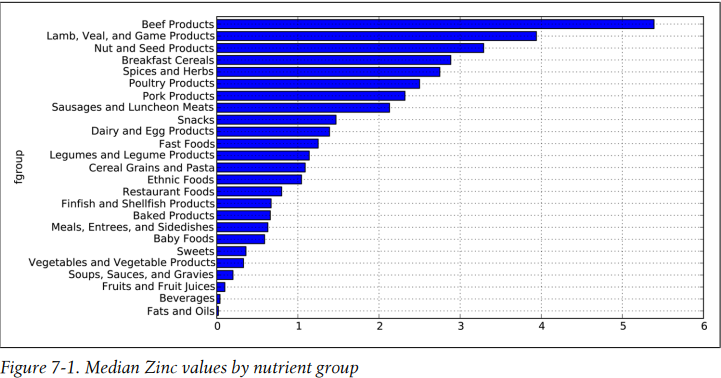
\includegraphics[scale=1.3]{Images/figure.png}
\par\textup{Hiển thị chất dinh dưỡng Animo Acid's ở DataFrame}
\par\quad\textup{In[284]: max\_foods.ix['Amino Acids']['food']}
\par\quad\textup{Out[284]:}
\par\quad\begin{tabular}{ll}
nutrient\\
Alanine &Gelatins, dry powder, unsweetened\\
Arginine& Seeds, sesame flour, low-fat\\
Aspartic& acid Soy protein isolate\\
Cystine& Seeds, cottonseed flour, low fat (glandless)\\
Glutamic acid& Soy protein isolate\\
Glycine& Gelatins, dry powder, unsweetened\\
Histidine& Whale, beluga, meat, dried (Alaska Native)\\
Hydroxyproline& KENTUCKY FRIED CHICKEN, Fried Chicken, ORIGINAL R\\
Isoleucine& Soy protein isolate, PROTEIN TECHNOLOGIES INTERNA\\
Leucine& Soy protein isolate, PROTEIN TECHNOLOGIES INTERNA\\
Lysine& Seal, bearded (Oogruk), meat, dried (Alaska Nativ\\
Methionine& Fish, cod, Atlantic, dried and salted\\
Phenylalanine& Soy protein isolate, PROTEIN TECHNOLOGIES INTERNA\\
Proline& Gelatins, dry powder, unsweetened\\
Serine &Soy protein isolate, PROTEIN TECHNOLOGIES INTERNA\\
Threonine& Soy protein isolate, PROTEIN TECHNOLOGIES INTERNA\\
Tryptophan& Sea lion, Steller, meat with fat (Alaska Native)\\
Tyrosine &Soy protein isolate, PROTEIN TECHNOLOGIES INTERNA\\
Valine& Soy protein isolate, PROTEIN TECHNOLOGIES INTERNA\\
Name: food

\par\end{tabular}
